% Provenance (never printed): see sources/outline_sources.md (Year 2: mid-latitude cyclones and
% fronts; jets and Rossby waves, descriptive; tropical cyclones; numerical weather prediction,
% principle). Definitions after the NWS glossary and UCAR; cyclogenesis conditions after the NOAA
% AOML FAQ; potential intensity after Gilford (2021, pyPI); conveyor belts after Raveh-Rubin and
% Catto (2019); blocking after Wang and others (2026); predictability after Krishnamurthy (2019),
% Selz and others (2022) and ECMWF. The Lorenz system from figdata/bachelor-2/weather.py; the
% fronts, waves and storms of the examples, exercises and problem are invented, their values
% computed in the Book 4 scratch calculator calc/ch22.py.
\chapter{الأنظمة الجوية}\label{ch:b2:weather-systems}

صار التنبّؤ لأربعة أيام قادمة اليوم بدقّة التنبّؤ ليوم واحد قبل ثلاثين
سنة، وأضاف كلّ عقد نحو يوم من التنبّؤ المفيد. ومع ذلك لا يُعوَّل على أيّ تنبّؤ بطقس
يوم معيّن، في مكان معيّن، أبعد كثيرًا من عشرة أيام، ولن تدفع الحواسيب الأفضل
وحدها ذلك الحدّ بعيدًا: فالغلاف الجوي يضخّم شكوكه الصغيرة. يصف هذا
الفصل الأنظمة الجوية التي تتتبّعها التنبّؤات، أي جبهات العروض الوسطى ومنخفضاتها،
وأمواج التيّار النفّاث والأعاصير المدارية، ثم الطريقة التي
يُتنبّأ بها ولماذا يجب أن يتوقّف التنبّؤ عند حدّ ما.
% ledger: mo:accuracy, bauer:day-per-decade, krish19:predictability

\begin{recall}
\textbf{من مجلّدات المدرسة}: الكتل الهوائية، والجبهات، والجبهات الباردة والدافئة، والمنخفضات
والمرتفعات الجوية، وخطوط تساوي الضغط والتنبّؤات الجوية؛ والإعصار المداري، وعينه وجدار عينه،
وسلّم سافير--سيمبسون. \textbf{من مجلد السنة الأولى}: قوّة تدرّج الضغط،
ومعامل كوريوليس $f = 2\Omega\sin\varphi$، والتوازن الجيوستروفي، والمنخفضات والمرتفعات،
والخلايا الثلاث، والرياح الغربية والتيّارات النفّاثة. \textbf{من كتب الفيزياء}: المحرّكات الحرارية
ومردود دورة كارنو. \textbf{من \cref{ch:b2:atmospheric-thermodynamics}}:
التشبّع، \omterm{def:b2:atmospheric-thermodynamics:moist-adiabat}{والمنحنى الأديباتي الرطب}، و$\theta_e$، \omterm{def:b2:atmospheric-thermodynamics:instability}{وعدم الاستقرار المشروط} وCAPE.
\end{recall}

\section{الجبهات}\label{sec:b2:weather-systems:fronts}

رسمت مجلّدات المدرسة الجبهات خطوطًا على الخريطة. والجبهة هي الخطّ الذي يلتقي فيه حدّ مائل
بين كتلتين هوائيتين بالأرض، ومن ذلك الميل يأتي طقسها.

\begin{definition}[السطح الجبهي؛ الجبهة الثابتة؛ الجبهة المسدودة]\label{def:b2:weather-systems:fronts}
\emph{السطح الجبهي}\index{السطح الجبهي} لجبهة هو الحدّ المائل بين
الكتلتين الهوائيتين، وترقد الكتلة الأكثف والأبرد تحته على شكل إسفين؛ والجبهة على الخريطة هي
تقاطعه مع الأرض. و\emph{الجبهة الثابتة}\index{الجبهة الثابتة} جبهة
تتحرّك ببطء شديد أو لا تتحرّك إطلاقًا. و\emph{الجبهة المسدودة}\index{الجبهة المسدودة}
جبهة مركّبة من جبهتين، تتكوّن حين تلحق جبهة باردة بجبهة دافئة أو ثابتة.
\end{definition}
% ledger: nws4:front, nws4:stationary, nws4:occluded

تتكوّن \omterm{def:b2:weather-systems:fronts}{الجبهة الثابتة} حين لا تستطيع أيّ من الكتلتين دفع الأخرى، فتهبّ الرياح على امتداد
الجبهة لا عبرها؛ وقد تبقى أيامًا، غائمة ممطرة، قبل أن تتحرّك من جديد جبهةً باردة
أو دافئة. وعلى الخريطة تتناوب فيها المثلّثات الزرقاء للجبهة الباردة، المتّجهة نحو
الهواء الدافئ، مع أنصاف الدوائر الحمراء للجبهة الدافئة، المتّجهة نحو الهواء البارد. أمّا \omterm{def:b2:weather-systems:fronts}{الجبهة
المسدودة} فتُرسم بالبنفسجي مع الرمزين كليهما على الجانب نفسه. فحين يكون الهواء خلف الجبهة الباردة
هو الأبرد، ينزلق تحت الجبهة الدافئة ويرفعها إلى الأعلى، وهذا انسداد بارد؛ وحين يكون الهواء
أمام الجبهة الدافئة هو الأبرد، تصعد الجبهة الباردة فوقه، وهذا انسداد دافئ.
% ledger: ucar4:stationary-occluded, nws4:occluded

ما مدى انحدار \omterm{def:b2:weather-systems:fronts}{السطح الجبهي}؟ يجمع الجواب التوازن الهيدروستاتيكي إلى التوازن
الجيوستروفي في مجلد السنة الأولى.

\begin{proposition}[ميل السطح الجبهي]\label{prop:b2:weather-systems:slope}
ليفصل سطح جبهي هواءً باردًا عند درجة الحرارة $T_c$ عن هواء دافئ عند $T_w$، مع
رياح جيوستروفية $v_c$ و$v_w$ على امتداد الجبهة. خذ المحور $x$ عبر الجبهة نحو
الهواء البارد والمحور $y$ على امتدادها، بحيث تكون الثلاثية $(x, y, z)$ يمنى. عندئذ يرتفع \omterm{def:b2:weather-systems:fronts}{السطح
الجبهي} نحو الهواء البارد بالميل
\[
  \tan\alpha \approx \frac{f\,\bar T\,(v_c - v_w)}{g\,(T_w - T_c)},
\]
حيث $\bar T$ درجة الحرارة المتوسطة. \omterm{def:b2:weather-systems:fronts}{فالسطح الجبهي} المتوازن يحتاج إلى قفزة في الريح
على امتداده، $v_c > v_w$: أي تدور الريح دورانًا إعصاريًّا عبر الجبهة.
\end{proposition}

\begin{proof}
الضغط متّصل عبر \omterm{def:b2:weather-systems:fronts}{السطح الجبهي}، فتغيّره على امتداد السطح هو
نفسه محسوبًا على أيّ من الجانبين: $\partial_x p_c\,\mathrm{d}x + \partial_z p_c\,\mathrm{d}z =
\partial_x p_w\,\mathrm{d}x + \partial_z p_w\,\mathrm{d}z$. وعلى كلّ جانب $\partial_z p = -\rho g$
(التوازن الهيدروستاتيكي) و$\partial_x p = \rho f v$ (التوازن الجيوستروفي). ومن ثَمّ
$\rho_c f v_c\,\mathrm{d}x - \rho_c g\,\mathrm{d}z = \rho_w f v_w\,\mathrm{d}x - \rho_w
g\,\mathrm{d}z$، و
\[
  \frac{\mathrm{d}z}{\mathrm{d}x} = \frac{f(\rho_c v_c - \rho_w v_w)}{g(\rho_c - \rho_w)} .
\]
وعند الضغط نفسه، $\rho \propto 1/T$، فيكون $\rho_c - \rho_w \approx \bar\rho\,(T_w -
T_c)/\bar T$؛ ويمكن في البسط إهمال الفرق الصغير بين الكثافتين، فنحصل
على الصيغة. والهواء البارد يرقد تحت، فيرتفع السطح نحوه، $\mathrm{d}z/
\mathrm{d}x > 0$، و$v_c > v_w$. ومع توجيه $x$ نحو الهواء البارد، تكون الدوّامية النسبية
$\partial v/\partial x$ عبر الجبهة عندئذ موجبة: أي إعصارية.
\end{proof}

\begin{example}[ميل نموذجي]\label{ex:b2:weather-systems:slope}
عند \ang{45} شمالًا، $f = \qty{1.03e-4}{s^{-1}}$. وعبر جبهة فيها $\bar T = \qty{280}{K}$، وفرق
حرارة قدره \qty{5}{K} وريح تتغيّر بمقدار \qty{10}{m/s} على امتدادها، يكون $\tan\alpha
= 1.03 \times 10^{-4} \times 280 \times 10/(9.81 \times 5) = 0.0059$، أي نحو 1 من 170: فيبلغ
\omterm{def:b2:weather-systems:fronts}{السطح الجبهي} ارتفاع \qty{1}{km} على بعد نحو \qty{170}{km} من الجبهة على الأرض.
وتغيّر أحدّ في الريح يعطي سطحًا أشدّ انحدارًا؛ وفرق أقوى في الحرارة يعطي سطحًا ألطف.
\end{example}

للجبهات الحقيقية ميول من هذه الرتبة، والإسفين الضحل يفسّر طقسها. فأمام
الجبهة الدافئة ينزلق الهواء الدافئ صاعدًا على منحدر لطيف مئات الكيلومترات: فتصل السحب العالية،
السمحاق والسمحاق الطبقي، أوّلًا، ثم الطبقي المتوسط، وتتكاثف السحب وتنخفض حتى
يبدأ المطر قرب الجبهة. أمّا الجبهة الباردة، الأشدّ انحدارًا والأسرع، حتى ضعف سرعة الجبهة
الدافئة، فترفع الهواء الدافئ فجأة: ركام وركام مزني، وزخّات، وهبّات وانخفاض مفاجئ
في الحرارة، مع ضغط يكفّ عن الانخفاض ويبدأ بالارتفاع حين تمرّ الجبهة. والجبهة
التي ينزل فيها الهواء الدافئ على \omterm{def:b2:weather-systems:fronts}{السطح الجبهي} بدل أن يصعد عليه تُسمّى جبهة هابطة.
% ledger: ucar:warm-front, ucar:cold-front, nws4:front

\begin{omfigure}
\centering
\begin{tikzpicture}[font=\scriptsize, >=Stealth, x=1cm, y=1cm]
% air masses
\fill[omCold!12] (0,0) -- (0,3.4) .. controls (1.6,2.2) and (3.2,0.8) .. (4,0) -- cycle;
\fill[omCold!12] (9.6,0) .. controls (11,0.6) and (12.6,1.5) .. (14,2.4) -- (14,0) -- cycle;
\fill[omWarm!8] (4,0) .. controls (3.2,0.8) and (1.6,2.2) .. (0,3.4) -- (0,4.8) -- (14,4.8)
  -- (14,2.4) .. controls (12.6,1.5) and (11,0.6) .. (9.6,0) -- cycle;
% frontal surfaces
\draw[omCold, thick] (4,0) .. controls (3.2,0.8) and (1.6,2.2) .. (0,3.4);
\draw[omWarm, thick] (9.6,0) .. controls (11,0.6) and (12.6,1.5) .. (14,2.4);
% clouds
\fill[black!18, draw=black!45] (3.75,0.5) .. controls (3.5,1.8) and (3.7,3.2) .. (3.9,3.9)
  .. controls (3.2,4.15) and (3.0,4.5) .. (3.4,4.6) -- (5.8,4.6) .. controls (6.1,4.45) and
  (5.7,4.15) .. (5.1,3.9) .. controls (5.3,3.0) and (5.4,1.6) .. (5.05,0.5) -- cycle;
\node[align=center] at (4.45,2.6) {ركام\\مزني};
\fill[black!15, draw=black!40] (9.6,0.35) .. controls (10.4,0.75) and (11.2,1.05) .. (11.9,1.25)
  -- (11.9,1.75) .. controls (11,1.6) and (10.2,1.35) .. (9.4,0.95) -- cycle;
\node at (10.75,1.25) [rotate=21] {مزن طبقي};
\fill[black!10, draw=black!35] (11.9,1.35) .. controls (12.3,1.55) and (12.7,1.75) .. (13.0,1.9)
  -- (13.0,2.25) .. controls (12.6,2.1) and (12.2,1.95) .. (11.9,1.85) -- cycle;
\node[anchor=south] at (12.45,2.15) {طبقي متوسط};
\draw[black!40, line width=1.6pt] (12.9,2.75) -- (13.9,3.05);
\node[anchor=south] at (13.35,3.05) {سمحاق طبقي};
\foreach \x in {12.2,12.7,13.2,13.7} {\draw[black!40, thick] (\x,3.95) .. controls (\x+0.15,4.05) .. (\x+0.35,3.9);}
\node[anchor=south] at (13.0,4.05) {سمحاق};
% rain
\foreach \x in {3.95,4.25,4.55,4.85} {\draw[omCold!70, dashed] (\x,0.45) -- (\x-0.12,0.02);}
\foreach \x in {9.8,10.2,10.6,11.0,11.4} {\draw[omCold!70, dashed] (\x,0.55) -- (\x-0.12,0.02);}
% ground and labels
\draw[thick] (0,0) -- (14,0);
\node at (1.2,0.8) {هواء بارد};
\node at (7.0,2.4) {القطاع الدافئ};
\node at (12.8,0.55) {هواء بارد};
\node[anchor=north, omCold] at (4,-0.05) {جبهة باردة};
\node[anchor=north, omWarm] at (9.6,-0.05) {جبهة دافئة};
\draw[->, thick] (6.0,0.55) -- (7.2,0.55) node[right] {الجبهات تتحرّك شرقًا};
\draw[->, black!60] (5.8,1.1) .. controls (7.0,1.4) and (9.5,2.0) .. (12.2,3.3);
\node[black!60, rotate=13] at (8.4,2.0) {الهواء الدافئ ينزلق صاعدًا};
\end{tikzpicture}
\par\smallskip{\small مقطع عرضي عبر جبهة باردة وجبهة دافئة، والغرب يسارًا
(تخطيطي: المقياس الرأسي مبالغ فيه نحو مئة مرّة، والجبهة الباردة مرسومة
أشدّ انحدارًا من الدافئة). أسماء السحب وتتابعها كما في النصّ.}
\end{omfigure}
% ledger: ucar:warm-front, ucar:cold-front

\section{الأعاصير خارج المدارية}\label{sec:b2:weather-systems:cyclones}

\begin{definition}[الإعصار خارج المداري؛ نموذج الجبهة القطبية؛ التكوّن الإعصاري]\label{def:b2:weather-systems:cyclones}
\emph{الإعصار خارج المداري}\index{الإعصار خارج المداري} إعصار من العروض الوسطى
والعليا، كثيرًا ما يبلغ عرضه نحو \qty{2000}{km}، ويحوي عادةً جبهات، منها جبهة باردة تمتدّ
مئات الكيلومترات نحو خطّ الاستواء. و\emph{نموذج الجبهة القطبية}\index{نموذج الجبهة القطبية}
يصف حياته موجةً تنمو على الجبهة القطبية، الجبهة الطويلة بين الهواء القطبي
والهواء المداري. و\emph{التكوّن الإعصاري}\index{التكوّن الإعصاري} هو نشوء
إعصار أو اشتداده.
\end{definition}
% ledger: nws4:extratropical, nws4:polar-front

يتتبّع النموذج الإعصار عبر أربع مراحل، كما يرسمها الشكل أدناه. جبهة ثابتة
تفصل هواءً باردًا يتحرّك غربًا على جانبها القطبي عن هواء دافئ يتحرّك شرقًا على جانبها
الاستوائي. ويثني اضطرابٌ الجبهةَ إلى موجة؛ فينخفض الضغط عند قمّتها، ويتكوّن
منخفض، وتتقدّم الجبهة شرق المنخفض نحو القطب جبهةً دافئة بينما تتقدّم الجبهة غربه
نحو خطّ الاستواء جبهةً باردة. وبينهما يقع القطاع الدافئ. والجبهة الباردة
أسرع من الدافئة، فيضيق القطاع الدافئ، وتلحق الجبهة الباردة بالدافئة
قرب المنخفض: فيمتدّ الانسداد إلى الخارج من المركز، رافعًا الهواء الدافئ عن
الأرض، ويمتلئ الإعصار، وقد انقطع عنه إمداد الهواء الدافئ، ويموت. وتُسمّى النقطة التي
تلتقي فيها الجبهات الثلاث النقطة الثلاثية. وفي صور الأقمار الصناعية يُظهر الإعصار الناضج
سحابة على شكل فاصلة، وشقًّا جافًّا من الهواء الصافي يلتفّ في جانبيه الجنوبي والشرقي.
% ledger: nws4:extratropical, nws4:occluded, ucar:cold-front

\begin{omfigure}
\centering
\begin{tikzpicture}[font=\scriptsize, >=Stealth]
% (a) stationary front
\begin{scope}[shift={(0,4.1)}]
\draw[black!30] (0,0) rectangle (6.4,3.4);
\node[anchor=north west] at (0,3.4) {\textbf{أ}\enspace جبهة ثابتة};
\draw[stationary front] (6.1,1.6) -- (0.3,1.6);
\draw[->, black!60] (4.2,2.5) -- (2.2,2.5); \node[black!60] at (3.2,2.8) {هواء بارد};
\draw[->, black!60] (2.2,0.7) -- (4.2,0.7); \node[black!60] at (3.2,0.4) {هواء دافئ};
\end{scope}
% (b) open wave
\begin{scope}[shift={(6.9,4.1)}]
\draw[black!30] (0,0) rectangle (6.4,3.4);
\node[anchor=north west] at (0,3.4) {\textbf{ب}\enspace موجة ومنخفض};
\fill[omWarm!10] (3.0,1.9) .. controls (3.9,1.75) and (4.8,1.55) .. (6.0,1.4) -- (6.0,0.2)
  -- (1.3,0.2) .. controls (2.0,0.9) and (2.6,1.4) .. (3.0,1.9) -- cycle;
\draw[black!45] (3.0,1.9) ellipse (0.55 and 0.4);
\draw[black!45] (3.0,1.9) ellipse (1.05 and 0.75);
\draw[warm front] (3.0,1.9) .. controls (3.9,1.75) and (4.8,1.55) .. (6.0,1.4);
\draw[cold front] (3.0,1.9) .. controls (2.6,1.4) and (2.0,0.9) .. (1.3,0.2);
\node[font=\small\bfseries, omWarm!70!black] at (2.7,2.15) {م};
\node at (4.5,0.75) {القطاع الدافئ};
\end{scope}
% (c) mature
\begin{scope}[shift={(0,0)}]
\draw[black!30] (0,0) rectangle (6.4,3.4);
\node[anchor=north west] at (0,3.4) {\textbf{ج}\enspace إعصار ناضج};
\fill[omWarm!10] (3.0,1.9) .. controls (3.9,1.7) and (4.8,1.5) .. (6.0,1.25) -- (6.0,0.2)
  -- (3.3,0.2) .. controls (3.3,0.8) and (3.2,1.45) .. (3.0,1.9) -- cycle;
\draw[black!45] (3.0,1.9) ellipse (0.5 and 0.36);
\draw[black!45] (3.0,1.9) ellipse (0.95 and 0.66);
\draw[black!45] (3.0,1.9) ellipse (1.4 and 0.95);
\draw[warm front] (3.0,1.9) .. controls (3.9,1.7) and (4.8,1.5) .. (6.0,1.25);
\draw[cold front] (3.0,1.9) .. controls (3.2,1.45) and (3.3,0.8) .. (3.3,0.2);
\node[font=\small\bfseries, omWarm!70!black] at (2.7,2.15) {م};
\node at (4.9,0.65) {القطاع الدافئ};
\end{scope}
% (d) occluded
\begin{scope}[shift={(6.9,0)}]
\draw[black!30] (0,0) rectangle (6.4,3.4);
\node[anchor=north west] at (0,3.4) {\textbf{د}\enspace الانسداد};
\fill[omWarm!10] (4.0,1.55) .. controls (4.6,1.45) and (5.3,1.3) .. (6.1,1.1) -- (6.1,0.2)
  -- (4.6,0.2) .. controls (4.5,0.7) and (4.3,1.2) .. (4.0,1.55) -- cycle;
\draw[black!45] (2.5,1.95) ellipse (0.5 and 0.36);
\draw[black!45] (2.5,1.95) ellipse (0.95 and 0.66);
\draw[black!45] (2.5,1.95) ellipse (1.45 and 0.95);
\draw[occluded front] (2.5,1.95) .. controls (3.0,1.9) and (3.6,1.75) .. (4.0,1.55);
\draw[warm front] (4.0,1.55) .. controls (4.6,1.45) and (5.3,1.3) .. (6.1,1.1);
\draw[cold front] (4.0,1.55) .. controls (4.3,1.2) and (4.5,0.7) .. (4.6,0.2);
\node[font=\small\bfseries, omWarm!70!black] at (2.2,2.2) {م};
\node[anchor=north east, align=right, fill=white, inner sep=1pt] at (3.9,1.3) {النقطة\\الثلاثية};
\fill (4.0,1.55) circle (0.6mm);
\end{scope}
\end{tikzpicture}
\par\smallskip{\small حياة إعصار خارج مداري في \omterm{def:b2:weather-systems:cyclones}{نموذج الجبهة القطبية}، في النصف
الشمالي، والشمال في الأعلى (تخطيطي): جبهة ثابتة (أ)؛ موجة ومنخفض عند قمّتها،
وجبهة دافئة وجبهة باردة والقطاع الدافئ بينهما (ب)؛ الجبهة الباردة تلحق
(ج)؛ \omterm{def:b2:weather-systems:fronts}{الجبهة المسدودة} تنمو من المركز (د). الحرف م: المنخفض؛ الأشكال البيضاوية السوداء: خطوط تساوي الضغط.}
\end{omfigure}
% ledger: nws4:occluded, nws4:extratropical, ucar4:stationary-occluded

ليست جبهات النموذج إلا الأثر السطحي للتيّارات الهوائية في الإعصار، التي
يصفها علماء الأرصاد بثلاثة تيّارات: الحزام الناقل الدافئ، أي الهواء الرطب الذي يصعد من
القطاع الدافئ أمام الجبهة الباردة؛ والحزام الناقل البارد على الجانب البارد من الجبهات؛
والتوغّل الجافّ، وهو تيّار من الهواء الآتي من أعالي التروبوسفير، وأحيانًا من أدنى
الستراتوسفير، ينزل نحو السطح خلف الجبهة الباردة وينتشر قرب
الأرض.
% ledger: rr19:conveyor

من أين تأتي طاقة الإعصار؟ لا من الحرارة الكامنة وحدها، كما في العاصفة الرعدية،
بل من فرق الحرارة بين الهواء القطبي والهواء المداري. فالأعاصير في العروض الوسطى
تشتدّ في المناطق الباروكلينية، حيث تتغيّر الحرارة أفقيًّا على سطح
ضغط ثابت وتتغيّر الريح مع الارتفاع. والإعصار النامي يحمل الهواء الدافئ نحو القطب
وإلى الأعلى والهواء البارد نحو خطّ الاستواء وإلى الأسفل: فيخفض مركز كتلة
الغلاف الجوي ويحوّل طاقة الوضع إلى طاقة حركية لرياحه. ويدرس مجلد السنة الثالثة
ذلك التحويل.
% ledger: nws4:extratropical

\begin{omfigure}
\centering
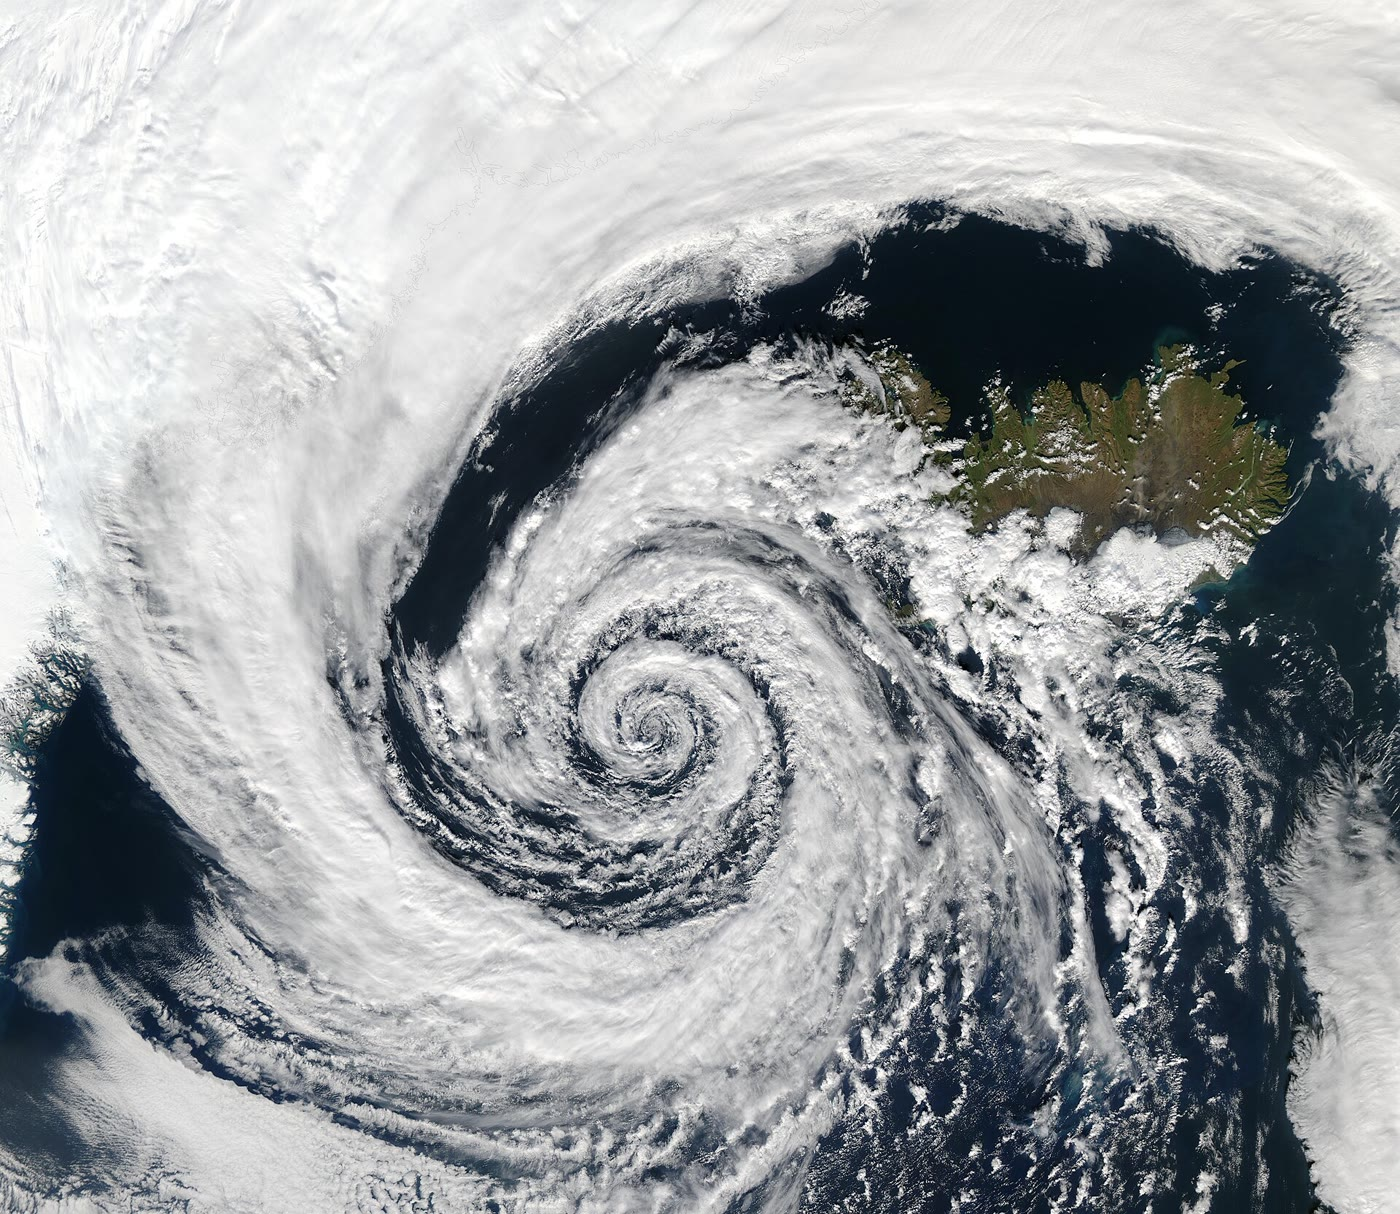
\includegraphics[width=0.58\linewidth]{images/book4/b2-22-iceland-low.jpg}
\par\smallskip{\small منخفض عميق قبالة الساحل الجنوبي الغربي لآيسلندا، 4 سبتمبر 2003، كما رآه
جهاز موديس على متن القمر الصناعي أكوا التابع لناسا: تلتفّ أشرطة السحب نحو المركز.
الصورة: \mbox{\textdir TLT NASA Goddard Space Flight Center, MODIS Rapid Response Team}،
\mbox{\textdir TLT Jacques Descloitres}، ملك عام، عبر \mbox{\textdir TLT Wikimedia Commons}.}
\end{omfigure}

\section{التيّارات النفّاثة وأمواج روسبي}\label{sec:b2:weather-systems:rossby}

لا تتوزّع الأعاصير عشوائيًّا. فالتيّار النفّاث القطبي، أي النواة السريعة للرياح الغربية فوق
الجبهة القطبية، يرافق موقع المرتفعات والمنخفضات في العروض الوسطى وحركتها؛
ويبلغ أقصى سرعته على امتداد نُواه، أي المقاطع التي تبلغ فيها سرعة ريحه ذروتها،
ولا يدور حول القطب حلقةً: بل يتعرّج.
% ledger: nws4:polar-front, nws4:jet-streak

\begin{definition}[موجة روسبي؛ الأخدود العلوي والحَيد العلوي]\label{def:b2:weather-systems:rossby}
\emph{موجة روسبي}\index{موجة روسبي} موجة في الجريان الغربي لأعالي التروبوسفير،
أي سلسلة من الأخاديد والحيود طولها آلاف الكيلومترات وسعتها بين الشمال والجنوب كبيرة.
و\emph{الأخدود العلوي}\index{الأخدود العلوي} منطقة مستطيلة ذات ضغط منخفض نسبيًّا
في مثل هذه الموجة، ينثني فيها الجريان نحو خطّ الاستواء؛ و\emph{الحَيد
العلوي}\index{الحَيد العلوي} منطقة مستطيلة ذات ضغط مرتفع نسبيًّا، ينثني فيها
نحو القطب.
\end{definition}
% ledger: nws4:rossby

توجد أمواج روسبي لأن معامل كوريوليس يزداد نحو القطب. فالهواء المدفوع نحو القطب
يجد $f$ أكبر، فيرتدّ نحو خطّ الاستواء محافظًا على دوّاميته المطلقة؛ والهواء
المدفوع نحو خطّ الاستواء يرتدّ نحو القطب. والمعدّل الذي يزداد به $f$ شمالًا،
$\beta = \mathrm{d}f/\mathrm{d}y = 2\Omega\cos\varphi/a$ حيث $a$ نصف قطر الأرض، يحدّد
سرعتها. ويشتقّ مجلد السنة الثالثة، من حفظ الدوّامية، سرعة الطور لموجة
طولها $\lambda$ في ريح غربية منتظمة $U$:
\[
  c = U - \frac{\beta}{k^2}, \qquad k = \frac{2\pi}{\lambda} .
\]
سلِّم بها هنا. فبالنسبة إلى الهواء، تتحرّك كلّ \omterm{def:b2:weather-systems:rossby}{موجة روسبي} غربًا، وكلّما طالت الموجة كانت
أسرع؛ والريح تحملها شرقًا. فالأمواج القصيرة تحملها الريح شرقًا بسرعة الريح تقريبًا،
والطويلة تنجرف ببطء، أو تثبت، أو حتى تتحرّك غربًا.
% ledger: earth:Trot, earth:Rmean

\begin{example}[ثلاث موجات عند خطّ العرض 45 شمالًا]\label{ex:b2:weather-systems:rossby}
مع $\Omega = \qty{7.292e-5}{s^{-1}}$ (يوم نجمي طوله \qty{23.9345}{h}) و$a =
\qty{6371}{km}$، يكون $\beta = \qty{1.62e-11}{m^{-1}.s^{-1}}$ عند \ang{45} شمالًا. وفي ريح غربية سرعتها
\qty{15}{m/s}، للموجة التي طولها \qty{4000}{km} القيمة $\beta/k^2 = \qty{6.6}{m/s}$ فتتحرّك شرقًا بسرعة
\qty{8.4}{m/s}؛ وللتي طولها \qty{6000}{km} القيمة $\beta/k^2 = \qty{14.8}{m/s}$ فتكاد لا تتحرّك، بسرعة
\qty{0.2}{m/s}؛ والتي طولها \qty{8000}{km} تتحرّك غربًا بسرعة \qty{11.2}{m/s}.
\end{example}
% ledger: earth:Trot, earth:Rmean

أخاديد الأمواج الطويلة تتحرّك ببطء وتدوم طويلًا؛ أمّا الأمواج القصيرة التي تعبرها،
أي الأخاديد القصيرة، فتحدث هواءً صاعدًا أمامها، على جانبها الشرقي، حيث
ينخفض الضغط السطحي وتنشأ المنخفضات. والأخدود الذي يميل محوره من الجنوب الشرقي إلى الشمال الغربي
علامة في الغالب على نظام ينشأ أو يشتدّ.
% ledger: nws4:rossby

\begin{omfigure}
\centering
\begin{tikzpicture}[font=\scriptsize, >=Stealth]
\foreach \lat/\pa in {30/-72, 45/-72, 60/-108} {
  \pgfmathsetmacro{\r}{6.0*tan((90-\lat)/2)}
  \draw[black!25] (0,0) circle (\r);
  \node[black!50, fill=white, inner sep=1pt] at (\pa:\r) {\foreignlanguage{arabic}{\mbox{\textdir TLT \ang{\lat}} شمالًا}};
}
\fill (0,0) circle (0.6mm);
\node[anchor=north, black!60] at (0,-0.08) {القطب الشمالي};
\draw[ocBlue, very thick, smooth, samples=241, domain=0:360]
  plot ({6.0*tan((90-(47+11*cos(5*\x)))/2)*cos(\x)}, {6.0*tan((90-(47+11*cos(5*\x)))/2)*sin(\x)});
\foreach \a in {18, 90, 162, 234, 306} {
  \pgfmathsetmacro{\ra}{6.0*tan((90-(47+11*cos(5*\a)))/2)}
  \pgfmathsetmacro{\rb}{6.0*tan((90-(47+11*cos(5*(\a+2))))/2)}
  \draw[ocBlue, very thick, -{Stealth[length=2.6mm]}] (\a:\ra) -- (\a+2:\rb);
}
\pgfmathsetmacro{\rt}{6.0*tan((90-36)/2)}
\node[anchor=216, ocRed!80!black, inner sep=2pt] at (36:\rt) {أخدود};
\node[anchor=0, ocRed!80!black, inner sep=2pt] at (180:\rt) {أخدود};
\pgfmathsetmacro{\rr}{6.0*tan((90-58)/2)}
\node[anchor=72, ocRed!80!black, inner sep=3pt] at (72:\rr) {حَيد};
\end{tikzpicture}
\par\smallskip{\small أمواج روسبي في التيّار النفّاث كما تُرى من فوق القطب الشمالي (تخطيطي):
خمس موجات حول نصف الكرة، تمتدّ الأخاديد نحو خطّ الاستواء والحيود نحو
القطب. يجري التيّار النفّاث شرقًا، عكس اتجاه عقارب الساعة كما يُرى من فوق القطب (الأسهم). ودوائر العرض
مرسومة كما على خريطة إسقاط مجسّم قطبي.}
\end{omfigure}
% ledger: nws4:rossby

وأحيانًا يتوقّف النمط عن الحركة تمامًا.

\begin{definition}[الحجب الجوّي]\label{def:b2:weather-systems:blocking}
\emph{الحجب الجوّي}\index{الحجب الجوّي} نظام ضغط مرتفع كبير ومستمرّ وشبه
ثابت، يقترن أحيانًا بمنخفض، يقطع الجريان الطبيعي للتيّار النفّاث نحو
الشرق. وتكاد طرائق رصد الحجب كلّها تشترط أن يدوم خمسة
أيام على الأقلّ.
\end{definition}
% ledger: wang26:blocking

يحرف الحجبُ التيّار النفّاث والأعاصير من حوله ويُبقي الطقس نفسه فوق المنطقة
نفسها أيامًا: فالحجب تجلب موجات الحرّ والجفاف وحرائق الغابات وموجات البرد والفيضانات إلى
العروض الوسطى. وفي أواخر يونيو وأوائل يوليو 2021 أدّى حجب قويّ إلى موجة الحرّ في
شمال غرب المحيط الهادئ من أمريكا الشمالية، التي سبّبت أكثر من ألف وفاة. والعمليات الفيزيائية
وراء الحجب لا تزال غير مفهومة جيّدًا، وتعجز النماذج العددية عن
إعادة إنتاج تكرار حدوث الحجب ومدّة بقائها.
% ledger: wang26:blocking, wang26:gaps

\section{الأعاصير المدارية}\label{sec:b2:weather-systems:tropical}

ليس للأعاصير المدارية جبهات ولا فرق حرارة تتغذّى عليه. فهي تستمدّ طاقتها
من المحيط الدافئ، عبر الحرارة الكامنة للماء الذي تبخّره، كما قاسها \cref{ch:b2:atmospheric-thermodynamics}.
وتساعد ستّة شروط على تكوّنها: ماء محيط لا تقلّ حرارته عن \qty{26.5}{\celsius}
حتى عمق من رتبة \qty{50}{m}؛ وغلاف جوي يبرد بسرعة كافية مع الارتفاع ليكون
غير مستقرّ للحمل الرطب؛ وتروبوسفير أوسط رطب، حول \qty{5}{km}؛ وبعد
لا يقلّ عن نحو \qty{500}{km} عن خطّ الاستواء، لتستطيع قوّة كوريوليس إبقاء المنخفض في
توازن؛ واضطراب سابق قرب السطح؛ وقصّ رأسي ضعيف للريح، أقلّ من نحو
\qty{10}{m/s} بين السطح وأعالي التروبوسفير. وهي ضرورية لكنها غير
كافية: فكثير من الاضطرابات التي تستوفيها لا تتطوّر أبدًا.
% ledger: aoml:tc-genesis

والإعصار المداري، متى تكوّن، محرّك حراري. فالهواء يلتفّ نحو الداخل فوق البحر عند حرارة شبه
ثابتة، مكتسبًا حرارة ورطوبة من المحيط؛ وفي جدار العين يصعد
أديباتيًّا؛ وفي التدفّق الخارج قرب التروبوبوز يفقد حرارة بالإشعاع عند حرارة منخفضة
شبه ثابتة؛ ثم يهبط ثانية بعيدًا عن المركز، فيكمل دورة
تشبه دورة كارنو. وشغل الدورة يدفع الرياح ضدّ احتكاك سطح
البحر.
% ledger: gilford21:pi

\begin{omfigure}
\centering
\begin{tikzpicture}[font=\scriptsize, >=Stealth, x=1cm, y=1cm]
% sea and axis
\fill[ocBlue!12] (0,-0.35) rectangle (12.5,0);
\draw[thick, ocBlue!70!black] (0,0) -- (12.5,0);
\node[anchor=north west, ocBlue!70!black] at (8.6,-0.02) {\foreignlanguage{arabic}{بحر دافئ، $T_s$}};
\draw[dashed, black!50] (0,-0.35) -- (0,4.9);
\node[anchor=south, black!60] at (0,4.9) {المركز};
% eyewall cloud and outflow cloud
\fill[black!14, draw=black!40] (0.9,0.25) .. controls (0.7,1.8) and (0.75,3.3) .. (0.95,4.2)
  .. controls (3.5,4.55) and (7.0,4.45) .. (9.5,4.2) .. controls (7.0,3.9) and (3.6,3.85)
  .. (2.1,3.7) .. controls (1.95,2.6) and (1.9,1.4) .. (2.0,0.25) -- cycle;
\node[black!60] at (0.45,2.0) [rotate=90] {العين};
\draw[black!50] (1.9,1.1) -- (2.45,1.1) node[anchor=west, black!70] {سحابة جدار العين};
% the cycle
\draw[->, very thick, ocRed] (11.4,0.3) -- (2.3,0.3);
\draw[->, very thick, ocRed] (1.45,0.45) .. controls (1.4,1.6) and (1.45,3.0) .. (1.75,4.0);
\draw[->, very thick, ocBlue] (2.2,4.25) -- (11.2,4.25);
\draw[->, very thick, ocBlue] (11.6,4.05) .. controls (11.75,2.8) and (11.75,1.5) .. (11.6,0.45);
\fill (11.6,0.3) circle (0.7mm) node[right=2pt] {A};
\fill (1.45,0.3) circle (0.7mm) node[left=2pt] {B};
\fill (1.8,4.25) circle (0.7mm) node[above left=1pt] {C};
\fill (11.6,4.25) circle (0.7mm) node[above right=1pt] {D};
\node[anchor=south, align=center] at (6.5,0.35) {\foreignlanguage{arabic}{\mbox{\textdir TLT A$\to$B}: تدفّق نحو الداخل فوق البحر عند نحو $T_s$،
  يكتسب الحرارة والرطوبة}};
\node[anchor=west, align=left] at (2.25,2.3) {\foreignlanguage{arabic}{\mbox{\textdir TLT B$\to$C}: صعود في جدار العين،}\\\foreignlanguage{arabic}{دون
  تبادل حرارة (منحنى أديباتي رطب)}};
\node[anchor=south, align=center] at (6.5,4.62) {\foreignlanguage{arabic}{\mbox{\textdir TLT C$\to$D}: تدفّق خارج قرب التروبوبوز عند نحو
  $T_o$، يفقد الحرارة بالإشعاع}};
\node[anchor=east, align=right] at (11.45,2.3) {\foreignlanguage{arabic}{\mbox{\textdir TLT D$\to$A}: هبوط بعيدًا}\\عن المركز};
\end{tikzpicture}
\par\smallskip{\small المحرّك الحراري للإعصار المداري، مقطع رأسي من المركز
إلى الخارج (تخطيطي، ليس على مقياس الرسم): تُكتسب الحرارة عند درجة حرارة سطح البحر
(A$\to$B) وتُعطى عند درجة الحرارة الأدنى بكثير للتدفّق الخارج (C$\to$D)، كما في دورة
كارنو.}
\end{omfigure}
% ledger: gilford21:pi

\begin{proposition}[الشدّة الكامنة]\label{prop:b2:weather-systems:pi}
\index{الشدّة الكامنة}
\emph{\omterm{prop:b2:weather-systems:pi}{الشدّة الكامنة}} لإعصار مداري، أي أقصى سرعة ريح قرب السطح يستطيع
المحيط والغلاف الجوي المحيطان به إدامتها، تُعطى تقريبًا بالعلاقة
\[
  V_{\max}^2 = \frac{C_k}{C_D}\,\frac{T_s - T_o}{T_o}\,\bigl(h_o^* - h^*\bigr),
\]
حيث $T_s$ درجة حرارة سطح البحر، و$T_o$ درجة حرارة التدفّق الخارج، و$C_k/C_D$
نسبة معاملَي تبادل الإنثالبي والزخم بين البحر والهواء،
وتؤخذ عادة 0.9، و$h_o^* - h^*$ زيادة $c_pT + gz + Lq$ عند التشبّع عند سطح
البحر على قيمتها عند التشبّع في الهواء فوق الطبقة الحدّية (مسلَّم بها).
\end{proposition}
% ledger: gilford21:pi

الكسر $(T_s - T_o)/T_o$ ليس مردود كارنو $(T_s - T_o)/T_s$ في كتب
الفيزياء: بل هو أكبر منه بالعامل $T_s/T_o$، لأن الاحتكاك الذي يبدّد الشغل يسخّن
الهواء المتدفّق نحو الداخل قرب سطح البحر، فيستعمل المحرّك تلك الحرارة ثانية. والعامل الأخير
هو الوقود. ففي غلاف جوي مداري تتبع حرارته \omterm{def:b2:atmospheric-thermodynamics:moist-adiabat}{المنحنى الأديباتي الرطب} لهواء
طبقته الحدّية، تكون $h^*$ قيمة $c_pT + gz + Lq$ في ذلك الهواء، ويقيس $h_o^* - h^*$
مدى بعد الهواء فوق البحر عن التشبّع عند حرارة البحر:
\[
  h_o^* - h^* \approx c_p\,(T_s - T_a) + L\,(q_s^* - q_a),
\]
حيث $T_a$ و$q_a$ درجة حرارة الهواء قرب السطح ورطوبته النوعية
و$q_s^*$ \omterm{def:b2:atmospheric-thermodynamics:moist-air}{الرطوبة النوعية} المشبعة عند درجة حرارة سطح البحر.
% ledger: gilford21:pi

\begin{example}[شدّة كامنة]\label{ex:b2:weather-systems:pi}
فوق بحر عند \qty{29}{\celsius} يكون الهواء عند \qty{1015}{hPa} في \qty{28}{\celsius} مع
رطوبة نسبية قدرها \qty{80}{\percent}، والتدفّق الخارج عند \qty{200}{K}، وهو متوسط سنوي
نموذجي فوق المحيطات المدارية الدافئة. ووفق \cref{prop:b2:atmospheric-thermodynamics:es,prop:b2:atmospheric-thermodynamics:humidity}،
$e_s(\qty{29}{\celsius}) = \qty{41.0}{hPa}$، فيكون $q_s^* = \qty{25.5}{g/kg}$، وللهواء، مع
$e = 0.8 \times \qty{38.7}{hPa}$، القيمة $q_a = \qty{19.2}{g/kg}$. ومن ثَمّ $h_o^* - h^* = 1004.5 \times
1 + 2.501 \times 10^6 \times 0.0063 = \qty{16.8}{kJ/kg}$، والعامل $(T_s - T_o)/T_o$ هو
$(302.15 - 200)/200 = 0.511$، و$V_{\max} = \sqrt{0.9 \times 0.511 \times 16\,800} =
\qty{88}{m/s}$.
\end{example}
% ledger: gilford21:pi

تقترب أقوى العواصف من مثل هذه القيم: فقمّة سلّم سافير--سيمبسون، الفئة
5، تبدأ عند \qty{70}{m/s}، وقد تجاوزت خمس عواصف حديثة \qty{86}{m/s}. ومعظم العواصف
نادرًا ما تبلغ شدّتها الكامنة: فالعواصف الحقيقية قلّما تكون في الحالة المستقرّة التي تفترضها
النظرية، والنظرية تُغفل القصّ الرأسي للريح، والهواء الجاف المسحوب إلى العاصفة
وهبوط الهواء من حولها، وكلّها تُضعف العاصفة.
% ledger: wk24:scale, gilford21:limits, aoml:tc-weaken

\begin{omfigure}
\centering
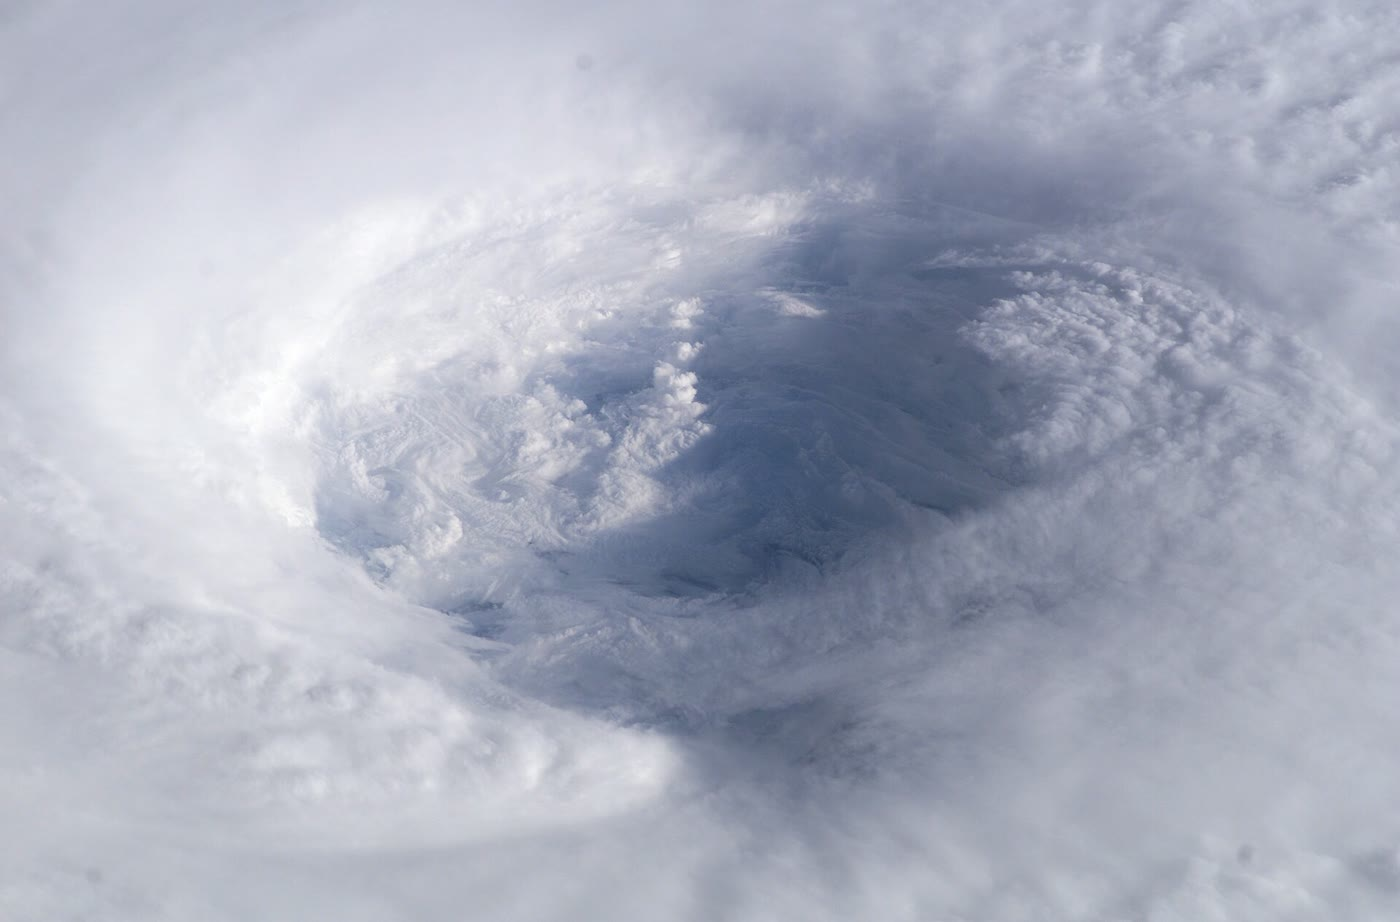
\includegraphics[width=0.62\linewidth]{images/book4/b2-22-isabel-eye.jpg}
\par\smallskip{\small عين الإعصار إيزابيل، 13 سبتمبر 2003، مصوَّرة من
محطّة الفضاء الدولية: ينحدر جدار العين كمدرّج ملعب نحو السحب المنخفضة في العين.
الصورة: رائد الفضاء في ناسا إد لو، ملك عام، عبر \mbox{\textdir TLT Wikimedia Commons}.}
\end{omfigure}

\section{التنبّؤ العددي بالطقس}\label{sec:b2:weather-systems:nwp}

\begin{definition}[التنبّؤ العددي بالطقس؛ تمثيل البيانات؛ التنبّؤ التجميعي؛ حدّ قابلية التنبّؤ]\label{def:b2:weather-systems:nwp}
\emph{التنبّؤ العددي بالطقس}\index{التنبّؤ العددي بالطقس} هو التنبّؤ
بالحاسوب: تُكامل المعادلات التي تحكم حركة الغلاف الجوي وطاقته وماءه
تقدّمًا في الزمن من حالته المرصودة. و\emph{تمثيل البيانات}\index{تمثيل البيانات}
يجمع أحدث الأرصاد إلى تنبّؤ قصير المدى انطلق من أرصاد
سابقة للحصول على أفضل تقدير للحالة الراهنة، أي التحليل، الذي ينطلق منه
التنبّؤ. و\emph{التنبّؤ التجميعي}\index{التنبّؤ التجميعي} مجموعة من التنبّؤات تُشغَّل
من حالات ابتدائية مختلفة قليلًا، وبصيغ مختلفة قليلًا من النموذج، لإظهار
مدى الطقس الممكن واحتماله. و\emph{حدّ قابلية
التنبّؤ}\index{حدّ قابلية التنبّؤ} هو الزمن الذي لا يعود بعده التنبّؤ بحالة
الطقس أفضل من تخمين مستمدّ من المناخ، لأن أخطاء الحالة الابتدائية
نمت حتى صارت بحجم الفروق بين أيّ حالتين للغلاف الجوي.
\end{definition}
% ledger: nws4:nwp, ecmwf4:da, ecmwf4:ens-fs, krish19:predictability

حُسب أوّل تنبّؤ عددي عام 1950 على حاسوب إنياك، أحد أوائل الحواسيب
الإلكترونية. ونموذج عالمي اليوم يقسم الغلاف الجوي إلى شبكة من خلايا عرض كلّ منها بضعة كيلومترات
وينطلق من تحليل يمزج أرصادًا من محطّات الأرصاد والطائرات
والمسابير اللاسلكية والسفن والعوّامات، وفوق كلّ شيء الأقمار الصناعية، التي تقدّم أكبر إسهام في
مهارة التنبّؤات العالمية. وفي أحد مراكز التنبّؤ الكبرى تضمّ المجموعة
51 عضوًا، تشغيلًا ضابطًا و50 تشغيلًا مضطربًا، بدقّة نحو \qty{9}{km}، تُشغَّل
مرّتين في اليوم حتى 15 يومًا مقبلة.
% ledger: krish19:predictability, ecmwf4:da, ecmwf4:ens

لماذا نُحدث اضطرابًا في تنبّؤ كان يمكن أن ينطلق من أفضل تحليل؟ لأن الغلاف الجوي
فوضوي، حسّاس لحالته الابتدائية. ونظام من ثلاثة متغيّرات، نُشر عام 1963، يبيّن ذلك
على أصغر مقياس.

\begin{proposition}[نظام لورنتز]\label{prop:b2:weather-systems:lorenz}
للنظام
\[
  \dot x = \sigma(y - x), \qquad \dot y = x(r - z) - y, \qquad \dot z = xy - bz,
\]
مع $\sigma = 10$ و$r = 28$ و$b = 8/3$، الخصائص الآتية.
\begin{enumerate}
  \item نقاطه الثابتة هي الأصل و$C_\pm = \bigl(\pm\sqrt{b(r - 1)}, \pm\sqrt{b(r - 1)},
        r - 1\bigr) = (\pm 8.49, \pm 8.49, 27)$.
  \item كلّ حجم في فضاء طوره يتقلّص بالشكل $\mathrm{e}^{-(\sigma + 1 + b)t}$: فتنتهي
        مساراته على مجموعة حجمها صفر، هي الجاذب.
  \item على الجاذب، يتباعد مساران يبدآن على مسافة صغيرة $\delta_0$ أحدهما من الآخر،
        في المتوسط، بالشكل $\delta(t) \approx \delta_0\,\mathrm{e}^{\lambda t}$، مع $\lambda =
        0.906$، حتى تبلغ $\delta$ حجم الجاذب (محسوب، ومسلَّم به). فالأخطاء الصغيرة
        تتضاعف كلّ $\ln 2/\lambda = 0.77$ وحدة زمنية.
\end{enumerate}
\end{proposition}
% ledger: nolitia22:lorenz

\begin{proof}[برهان 1 و2]
عند نقطة ثابتة، $y = x$ من المعادلة الأولى؛ والثالثة تعطي $z = x^2/b$؛ والثانية
تصبح $x(r - 1 - x^2/b) = 0$، فيكون $x = 0$ أو $x^2 = b(r - 1) = 72$. وتباعد
الحقل المتّجهي هو $\partial_x\dot x + \partial_y\dot y + \partial_z\dot z = -\sigma - 1 - b$، وهو
ثابت، وبمبرهنة التباعد يحقّق حجم $V$ يحمله الجريان العلاقة $\dot V =
-(\sigma + 1 + b)V$.
\end{proof}

تبيّن الأشكال معنى القضية. فتشغيلان يبدآن على بعد \num{e-5} أحدهما من الآخر يتبع أحدهما
الآخر نحو خمس عشرة وحدة زمنية، ثم يفترقان نهائيًّا: كلّ منهما لا يزال يبدو مسارًا
معقولًا للنظام، لكنهما لم يعودا المسار نفسه. وبأخذ المتوسط على 200 زوج من
التشغيلات بدأت على بعد \num{e-8}، تنمو المسافة أُسّيًّا بالمعدّل $\lambda$، أي خطًّا
مستقيمًا على مقياس لوغاريتمي، حتى تتشبّع عند حجم الجاذب. وأيًّا كان
الخطأ الابتدائي، فهو يبلغ ذلك الحجم: والخطأ الابتدائي الأصغر لا يفعل إلا أن يؤخّر اللحظة، بمقدار
$\ln 10/\lambda = 2.5$ وحدة زمنية لكلّ تخفيض بعشرة أضعاف.
% ledger: nolitia22:lorenz

\begin{omfigure}
\centering
% figdata/bachelor-2/weather.py parts traj, butterfly
\begin{tikzpicture}
\begin{groupplot}[group style={group size=2 by 1, horizontal sep=1.5cm},
  tick label style={font=\scriptsize}, label style={font=\small}]
\nextgroupplot[width=0.58\linewidth, height=5.0cm, xmin=0, xmax=30, ymin=-22, ymax=22,
  xlabel={الزمن}, ylabel={$x$}, legend style={font=\scriptsize, at={(0.5,1.02)},
  anchor=south, draw=none, legend columns=2, /tikz/every even column/.append style={column
  sep=0.4cm}}, legend cell align=left]
\addplot[ocBlue, thin] table[x=t, y=x1] {figdata/out/bachelor-2-weather-traj.dat};
\addlegendentry{\foreignlanguage{arabic}{التشغيل 1}}
\addplot[ocRed, thin, densely dashed] table[x=t, y=x2] {figdata/out/bachelor-2-weather-traj.dat};
\addlegendentry{\foreignlanguage{arabic}{التشغيل 2، بدأ على بعد \num{e-5} منه}}
\nextgroupplot[width=0.4\linewidth, height=5.0cm, xmin=-22, xmax=22, ymin=0, ymax=52,
  xlabel={$x$}, ylabel={$z$}]
\addplot[black!70, very thin] table[x=x, y=z] {figdata/out/bachelor-2-weather-butterfly.dat};
\addplot[only marks, mark=*, mark size=1.3pt, ocRed] coordinates {(8.485,27) (-8.485,27)};
\end{groupplot}
\end{tikzpicture}
\par\smallskip{\small نظام لورنتز ($\sigma = 10$، $r = 28$، $b = 8/3$)، مكاملًا بطريقة
رونغه--كوتا بخطوة زمنية قدرها 0.01. يسارًا: تشغيلان يبدآن على بعد \num{e-5} في $x$
على الجاذب. يمينًا: تشغيل واحد على مدى 40 وحدة زمنية، كما يُرى على امتداد $y$، مع النقطتين الثابتتين
$C_\pm$ (بالأحمر).}
\end{omfigure}
% ledger: nolitia22:lorenz

\begin{omfigure}
\centering
% figdata/bachelor-2/weather.py part growth
\begin{tikzpicture}
\begin{axis}[width=0.72\linewidth, height=5.6cm, xmin=0, xmax=30, ymode=log, ymin=1e-9,
  ymax=1e3, ytick={1e-9,1e-7,1e-5,1e-3,1e-1,1e1,1e3}, xlabel={الزمن}, ylabel={المسافة بين التشغيلين}, tick label style={font=\scriptsize},
  label style={font=\small}, legend style={font=\scriptsize, at={(0.02,0.98)}, anchor=north west,
  draw=none, fill=none}, legend cell align=left, unbounded coords=discard, grid=major,
  grid style={black!8}]
\addplot[ocBlue, line width=1.6pt, opacity=0.55] table[x=t, y expr=10^\thisrow{log10d}]
  {figdata/out/bachelor-2-weather-growth.dat};
\addlegendentry{\foreignlanguage{arabic}{متوسط 200 زوج (هندسي)}}
\addplot[black, densely dashed, thin] table[x=t, y expr=10^\thisrow{fit}]
  {figdata/out/bachelor-2-weather-growth.dat};
\addlegendentry{\foreignlanguage{arabic}{أسّية موفَّقة، من $t = 2$ إلى 16}}
\end{axis}
\end{tikzpicture}
\par\smallskip{\small نموّ المسافة بين أزواج من تشغيلات نظام لورنتز بدأت على بعد
\num{e-8}. يرتفع الخطّ الموفَّق بعامل عشرة كلّ 2.57 وحدة زمنية، أي بمعدّل 0.897؛
وأكبر أسّ لليابونوف، محسوبًا بإعادة تقييس زوج واحد على مدى 2000 وحدة زمنية، هو
0.909، مقابل 0.906 منشورًا. ويتوقّف النموّ عند حجم الجاذب.}
\end{omfigure}
% ledger: nolitia22:lorenz

يسلك الغلاف الجوي المسلك نفسه، بمتغيّرات أكثر بكثير وبأخطاء تنمو
بمعدّلات مختلفة على مقاييس مختلفة. فمن تنبّؤات ثمانينيات القرن العشرين، وُجد أن الأخطاء الصغيرة
تتضاعف في نحو 2.4 يوم، وأن التنبّؤ الموثوق بحالة الطقس يتوقّف دون
نحو عشرة أيام. والتجارب التي تقلّص شكّ الحالة الابتدائية اليوم، مع نموذج
مفترض كاملًا، تجد أن الشروط الابتدائية الكاملة لن تضيف إلا أربعة إلى خمسة أيام،
وأن تخفيضًا بنسبة 90 في المئة يعطي معظم ذلك سلفًا: فكلّما صغرت الأخطاء، نمت
أسرع، عبر تحرّر الحرارة الكامنة في الحمل، على مقاييس أصغر ممّا يستطيع التنبّؤ
تمييزه. ويقع \omterm{def:b2:weather-systems:nwp}{حدّ قابلية التنبّؤ} في العروض الوسطى حول أسبوعين. والتنبّؤات
تكسب نحو يوم كلّ عقد لأن الأرصاد \omterm{def:b2:weather-systems:nwp}{وتمثيل البيانات} والنماذج الأفضل تقرّبها
من ذلك الحدّ؛ لكنها لا تستطيع تجاوزه.
% ledger: krish19:predictability, selz22:limit, bauer:day-per-decade

\omterm{def:b2:weather-systems:nwp}{والتنبّؤ التجميعي} يحوّل هذا إلى أداة. فأعضاؤه ينطلقون من تحليلات تختلف بقدر
ما يكون التحليل نفسه غير مؤكّد؛ فما داموا متّفقين، يكون التنبّؤ حادًّا؛ وحين
يتباعدون، يجب أن يقول التنبّؤ ذلك، فيعطي احتمالات. ويُسمّى التنبّؤ موثوقًا حين
تقع الأحداث التي يعلنها باحتمال \qty{70}{\percent} في \qty{70}{\percent} من
الحالات.
% ledger: ecmwf4:ens-fs

\begin{inthelab}[يوم في مركز للتنبّؤ]
\begin{minipage}[t]{0.54\linewidth}\vspace{0pt}
في مركز عالمي للتنبّؤ يدور اليوم حول موعدين، الساعة 00 والساعة 12 بالتوقيت العالمي المنسّق. فتصل الأرصاد الصالحة
حول كلّ موعد بالملايين، من الأقمار الصناعية والمسابير اللاسلكية والطائرات والسفن
والعوّامات ومحطّات الأرصاد؛ ويمزجها \omterm{def:b2:weather-systems:nwp}{تمثيل البيانات} مع التنبّؤ القصير السابق في
التحليل. وتنطلق النماذج منه، \omterm{def:b2:weather-systems:nwp}{والتنبّؤ التجميعي} كذلك، وتصل التنبّؤات إلى مستعمليها
بعد ساعات عدّة، بعد أن تكون الحواسيب الفائقة قد حسبت 15 يومًا مقبلة. ثم يقارن المتنبّئون
التشغيلات، ويتحقّقون منها في ضوء أحدث الأرصاد وصور الأقمار الصناعية، ويتتبّعون
الأعاصير والجبهات، ويحوّلون احتمالات \omterm{def:b2:weather-systems:nwp}{التنبّؤ التجميعي} إلى إنذارات
وتنبّؤات.
\end{minipage}\hfill
\begin{minipage}[t]{0.42\linewidth}\vspace{0pt}
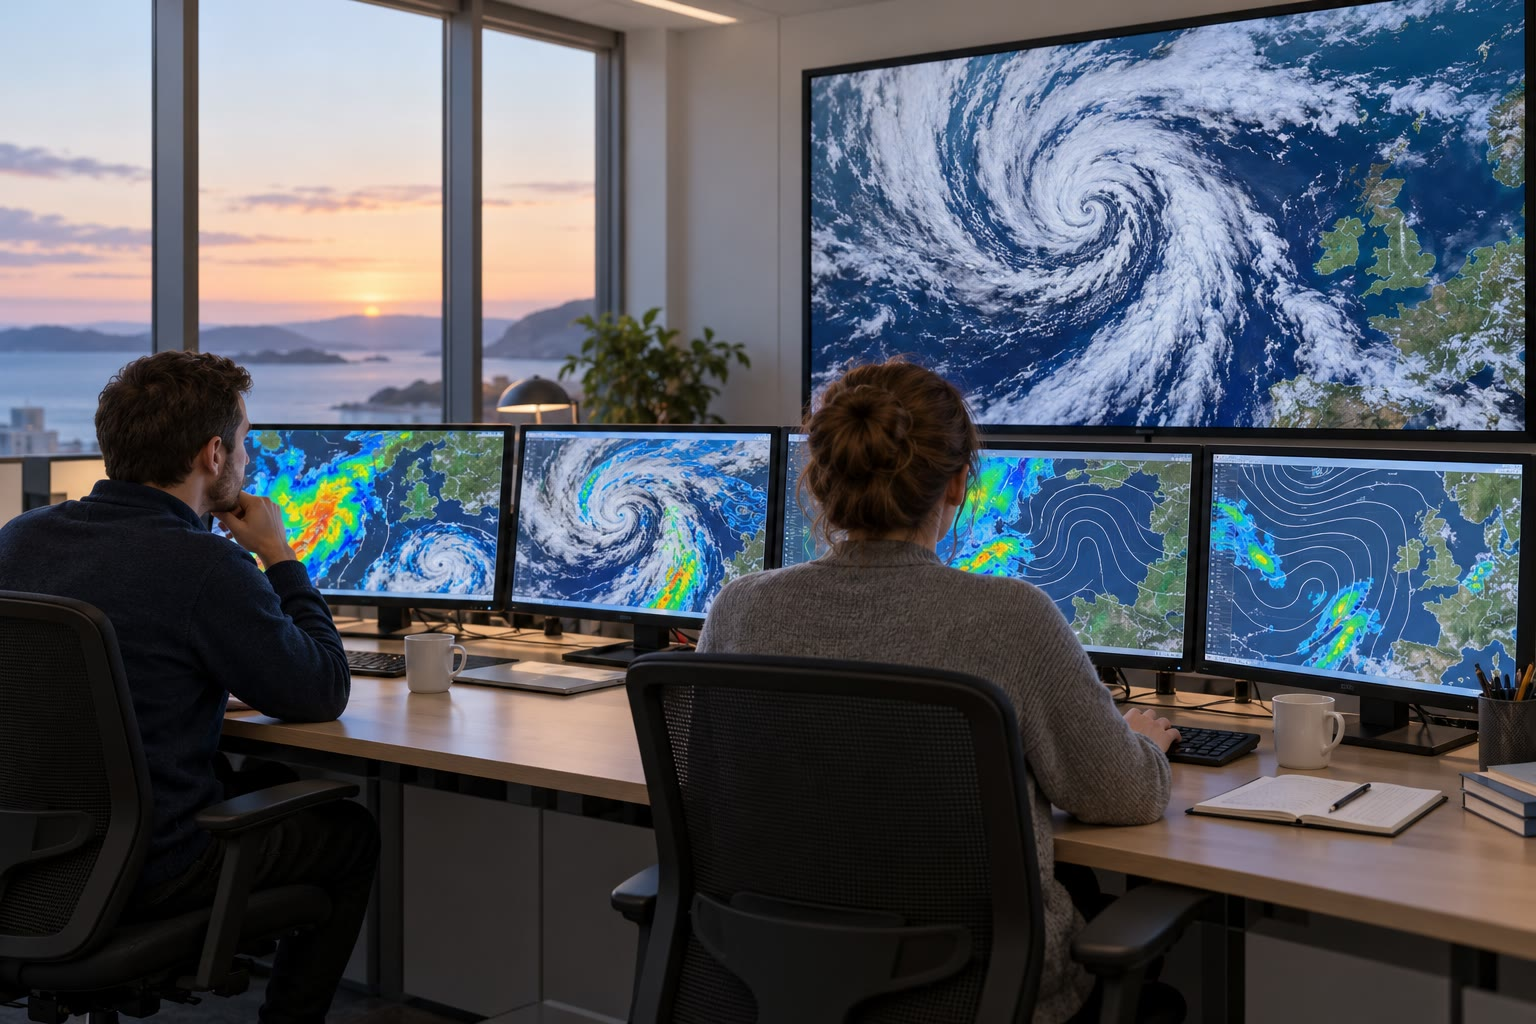
\includegraphics[width=\linewidth]{images/book4/ai/b2-forecast-office.jpg}

{\scriptsize متنبّئون يعملون أمام صور الأقمار الصناعية وخرائط النماذج
(رسم توضيحي مولَّد بالذكاء الاصطناعي).}
\end{minipage}
% ledger: ecmwf4:ens, ecmwf4:da, mo:how-forecasts
\end{inthelab}

\section*{التمارين}\label{sec:b2:weather-systems:exercises}

معطيات التمارين، ما لم يُذكر غير ذلك: $\Omega = \qty{7.292e-5}{s^{-1}}$، و$a =
\qty{6371}{km}$، و$g = \qty{9.81}{m.s^{-2}}$، و$c_p = \qty{1004.5}{J.kg^{-1}.K^{-1}}$، و$L =
\qty{2.501e6}{J/kg}$، \omterm{def:b2:atmospheric-thermodynamics:moist-air}{وضغط البخار} المشبع الوارد في تمارين
\cref{ch:b2:atmospheric-thermodynamics}.
% ledger: earth:Trot, earth:Rmean

\begin{exercise}[$\star$]\label{exo:b2:weather-systems:1}
عند \ang{50} شمالًا تفصل جبهة باردة هواءً عند \qty{275}{K} عن هواء عند \qty{281}{K}، وتتغيّر الريح
على امتدادها بمقدار \qty{15}{m/s}. (أ) احسب $f$. (ب) احسب ميل \omterm{def:b2:weather-systems:fronts}{السطح الجبهي}،
بالصيغة 1 من $N$. (ج) على أيّ مسافة خلف الجبهة على الأرض يبلغ \omterm{def:b2:weather-systems:fronts}{السطح الجبهي}
ارتفاع \qty{1}{km}؟ (د) ماذا يحدث للميل إذا تضاعف فرق الحرارة مع بقاء تغيّر
الريح نفسه؟
\end{exercise}

\begin{exercise}[$\star$]\label{exo:b2:weather-systems:2}
يرتفع سطح جبهي دافئ بميل 1 من 150 ويتحرّك بسرعة \qty{25}{km/h}. (أ) على أيّ مسافة أمام
الجبهة على الأرض يقع \omterm{def:b2:weather-systems:fronts}{السطح الجبهي} على ارتفاع \qty{6}{km}؟ (ب) يرى راصد سحبًا عالية تتكوّن
عليه هناك. بعد كم من الوقت تصل الجبهة إلى الراصد؟ (ج) صِف تتابع
السحب التي يراها الراصد في أثناء ذلك.
\end{exercise}
% ledger: ucar:warm-front

\begin{exercise}[$\star$]\label{exo:b2:weather-systems:3}
على خريطة لنصف الكرة الشمالي، (أ) خطّ عليه مثلّثات زرقاء على جانبه الجنوبي الشرقي يمتدّ نحو الجنوب الغربي
من منخفض؛ (ب) خطّ عليه أنصاف دوائر حمراء على جانبه الشمالي يمتدّ شرقًا من المنخفض نفسه؛ (ج)
خطّ بنفسجي يحمل الرمزين معًا يمتدّ من منخفض آخر إلى نقطة تبدأ منها جبهتان أخريان؛
(د) خطّ تتناوب عليه مثلّثات زرقاء على جانبه الجنوبي وأنصاف دوائر حمراء على جانبه الشمالي.
سمِّ كلّ جبهة، وبيّن أين الهواء البارد وفي أيّ اتجاه تتحرّك كلّ منها.
\end{exercise}
% ledger: ucar4:stationary-occluded, nws4:occluded

\begin{exercise}[$\star$]\label{exo:b2:weather-systems:4}
عند \ang{45} شمالًا في ريح غربية سرعتها \qty{12}{m/s}: (أ) احسب $\beta$. (ب) احسب سرعة الطور
لموجتين طولهما \qty{4000}{km} و\qty{8000}{km}. (ج) في أيّ اتجاه تتحرّك كلّ منهما، وما المسافة التي تقطعها في
يوم؟
\end{exercise}

\begin{exercise}[$\star\star$]\label{exo:b2:weather-systems:5}
(أ) بيّن أن \omterm{def:b2:weather-systems:rossby}{موجة روسبي} تثبت في ريح غربية $U$ حين يكون $\lambda = 2\pi\sqrt{U/\beta}$.
(ب) احسبه عند \ang{45} شمالًا مع $U = \qty{12}{m/s}$. (ج) كم موجة كهذه تتّسع لها دائرة
العرض؟ (د) لماذا ترجّح ريح غربية أقوى عددًا أقلّ من الموجات الثابتة الأطول؟
\end{exercise}

\begin{exercise}[$\star\star$]\label{exo:b2:weather-systems:6}
لنظام لورنتز: (أ) تحقّق من أن $C_+$ نقطة ثابتة بحساب المشتقّات الثلاث
عندها. (ب) بأيّ عامل يتقلّص حجم صغير من فضاء الطور في وحدة زمنية واحدة؟ (ج) لماذا
لا يمنع هذا مسارين متجاورين من التباعد؟
\end{exercise}

\begin{exercise}[$\star\star$]\label{exo:b2:weather-systems:7}
خذ $\lambda = 0.906$ لنظام لورنتز وحجمًا للجاذب قدره 10. (أ) احسب
زمن تضاعف الأخطاء الصغيرة. (ب) كم يستغرق خطأ قدره \num{e-8} ليبلغ حجم
الجاذب؟ (ج) بكم يؤخّر خطأ ابتدائي أصغر بألف مرّة تلك اللحظة؟ وما
الكسر الذي يمثّله ذلك من الزمن الذي وُجد في (ب)؟
\end{exercise}
% ledger: nolitia22:lorenz

\begin{exercise}[$\star\star$]\label{exo:b2:weather-systems:8}
بحر عند \qty{303}{K} تدفّقه الخارج عند \qty{195}{K}؛ وعدم التوازن هو $h_o^* - h^* =
\qty{15}{kJ/kg}$ و$C_k/C_D = 0.9$. (أ) احسب \omterm{prop:b2:weather-systems:pi}{الشدّة الكامنة}. (ب) قارنها
بعتبة الفئة 5 وبأسرع العواصف الحديثة. (ج) لماذا لا تبلغها معظم
العواصف؟
\end{exercise}
% ledger: gilford21:pi, wk24:scale

\begin{exercise}[$\star\star$]\label{exo:b2:weather-systems:9}
للعاصفة في \cref{exo:b2:weather-systems:8}: (أ) احسب مردود كارنو لمحرّك
يعمل بين سطح البحر والتدفّق الخارج. (ب) احسب العامل $(T_s - T_o)/T_o$ في
\cref{prop:b2:weather-systems:pi} والنسبة بينهما. (ج) فسّر الفرق.
\end{exercise}
% ledger: gilford21:pi

\begin{exercise}[$\star\star\star$]\label{exo:b2:weather-systems:10}
(أ) أعد اشتقاق \cref{prop:b2:weather-systems:slope}، محتفظًا بالكثافات الدقيقة، وبيّن أن
الهواء البارد يجب أن يقع في الأسفل. (ب) عبر منطقة جبهية عرضها \qty{50}{km} عند \ang{45} شمالًا تتغيّر الريح
على امتداد الجبهة بمقدار \qty{10}{m/s}. احسب الدوّامية النسبية للمنطقة وقارنها
بالمعامل $f$. (ج) هل المنطقة إعصارية أم ضدّ إعصارية؟
\end{exercise}

\begin{exercise}[$\star\star\star$]\label{exo:b2:weather-systems:11}
افترض أن أخطاء التنبّؤ تتضاعف كلّ 2.4 يوم، وتبدأ عند \qty{0.5}{K} وتصبح عديمة الجدوى عند
\qty{6}{K}. (أ) أوجد أفق التنبّؤات المفيدة. (ب) بأيّ عامل يجب أن يتقلّص الخطأ الابتدائي
كلّ عقد لكسب يوم في كلّ عقد، لو كان النموذج كاملًا؟ (ج) تجد التجارب أن
خطأً ابتدائيًّا أصغر بعشر مرّات لا يكسب إلا 4 إلى 5 أيام. أيّ زمن تضاعف يقتضيه ذلك
للأخطاء الصغيرة، وماذا يقول عن طريقة نموّ الأخطاء الصغيرة؟
\end{exercise}
% ledger: krish19:predictability, selz22:limit, bauer:day-per-decade

\begin{exercise}[$\star\star\star$]\label{exo:b2:weather-systems:12}
خذ \cref{ex:b2:weather-systems:pi} وسخّن البحر والهواء كليهما بمقدار \qty{1}{K}، مع بقاء
الرطوبة النسبية ودرجة حرارة التدفّق الخارج دون تغيير. (أ) أعد حساب $q_s^*$ و$q_a$
وعدم التوازن. (ب) أعد حساب \omterm{prop:b2:weather-systems:pi}{الشدّة الكامنة}. (ج) بكم في المئة لكل كلفن
ترتفع، وأيّ العوامل يسهم أكثر من غيره؟
\end{exercise}
% ledger: gilford21:pi

\begin{problem}[{مسألة نهاية الأسبوع --- إلى أيّ مدى مقبل؟}]\label{pb:b2:weather-systems:1}
تُظهر خريطة طقس مختلَقة عند \ang{50} شمالًا جبهة باردة تتقدّم نحو بلدة، وفوقها \omterm{def:b2:weather-systems:rossby}{موجة روسبي}
في التيّار النفّاث. تتبع المسألة الجبهة، ثم الموجة، ثم تسأل إلى أيّ مدى
مقبل يمكن التنبّؤ بأيّ من ذلك. استعمل معطيات التمارين.

\medskip\noindent\textbf{الجزء الأول --- الجبهة.}
في الساعة 06 بالتوقيت العالمي المنسّق تكون الجبهة الباردة على بعد \qty{480}{km} غرب البلدة، وفي الساعة 12 على بعد \qty{390}{km}. وخلفها
يكون الهواء عند \qty{277}{K}، وفي القطاع الدافئ عند \qty{285}{K}، وتتغيّر الريح على امتداد الجبهة
بمقدار \qty{16}{m/s} عبرها.
\begin{enumerate}
  \item أوجد سرعة الجبهة.
  \item في أيّ ساعة تصل إلى البلدة؟
  \item احسب $f$ عند \ang{50} شمالًا.
  \item احسب ميل \omterm{def:b2:weather-systems:fronts}{السطح الجبهي}.
  \item ما ارتفاع \omterm{def:b2:weather-systems:fronts}{السطح الجبهي} فوق البلدة بعد ستّ ساعات من مرور الجبهة؟
  \item بعد كم من الوقت من المرور يبلغ الهواء البارد ارتفاع \qty{1.5}{km} فوق البلدة؟
  \item ما الطقس الذي تشهده البلدة حين تمرّ الجبهة، وكيف يتغيّر الضغط؟
\end{enumerate}

\medskip\noindent\textbf{الجزء الثاني --- الموجة في الأعالي.}
في التيّار النفّاث فوقها، تبلغ سرعة الريح الغربية \qty{20}{m/s} وطول الموجة \qty{5000}{km}.
\begin{enumerate}[resume]
  \item احسب $\beta$ عند \ang{50} شمالًا.
  \item احسب $k$ و$\beta/k^2$.
  \item أوجد سرعة طور الموجة.
  \item ما المسافة التي يقطعها الأخدود في 24 ساعة؟
  \item أوجد طول الموجة الذي يثبت في هذه الريح، وكم موجة كهذه تتّسع لها
        دائرة العرض \ang{50} شمالًا.
  \item أين ينبغي أن يتعمّق الإعصار السطحي بالنسبة إلى \omterm{def:b2:weather-systems:rossby}{الأخدود العلوي}؟
\end{enumerate}

\medskip\noindent\textbf{الجزء الثالث --- غلاف جوي مصغَّر.}
في شكل نموّ الأخطاء في نظام لورنتز، يمرّ الخطّ الموفَّق بالقيمة
\num{5e-7} تقريبًا عند $t = 4$ وبالقيمة \num{3.9e-3} عند $t = 14$.
\begin{enumerate}[resume]
  \item من هاتين القراءتين، احسب معدّل النموّ $\lambda$.
  \item احسب زمن التضاعف.
  \item قارن بالأسّ المنشور 0.906.
  \item لماذا تتوقّف المسافة عن النموّ، عند نحو 15؟
  \item كم يتأخّر خطأ أصغر بعشر مرّات في بلوغ ذلك الحجم؟
\end{enumerate}

\medskip\noindent\textbf{الجزء الرابع --- إلى أيّ مدى مقبل؟}
خذ زمن التضاعف 2.4 يوم الذي وُجد للأخطاء الصغيرة في تنبّؤات ثمانينيات القرن العشرين،
وخطأً ابتدائيًّا قدره \qty{0.1}{\celsius} في درجة الحرارة عند مستوى ما، وتنبّؤًا يصبح
عديم الجدوى متى بلغ الخطأ \qty{3}{\celsius}.
\begin{enumerate}[resume]
  \item كم تضاعفًا يفصل الخطأ الابتدائي عن الخطأ الذي يجعل التنبّؤ عديم الجدوى؟
  \item كم يومًا يستغرق ذلك؟
  \item كم يومًا يكسب تنصيف الخطأ الابتدائي؟
  \item مع التقدير الأقدم لزمن تضاعف قدره 5 أيام، أيّ أفق يجده المرء؟
  \item تجد التجارب الحديثة أن خطأً ابتدائيًّا أصغر بعشر مرّات، بل حالةً
        ابتدائية كاملة، لا يكسب إلا 4 إلى 5 أيام. لماذا يوحي ذلك بأن تقدير
        السؤال 20 متفائل؟
  \item خلاصة القول: إلى أيّ مدى مقبل، بالأيام، يمكن أن يكون هذا التنبّؤ مفيدًا؟
\end{enumerate}
\end{problem}
% ledger: krish19:predictability, selz22:limit, nolitia22:lorenz, ucar:cold-front
